% file: 3-10-traversability/hierholzer.tex

\documentclass[tikz]{standalone}
\usetikzlibrary{positioning, chains}

\begin{document}
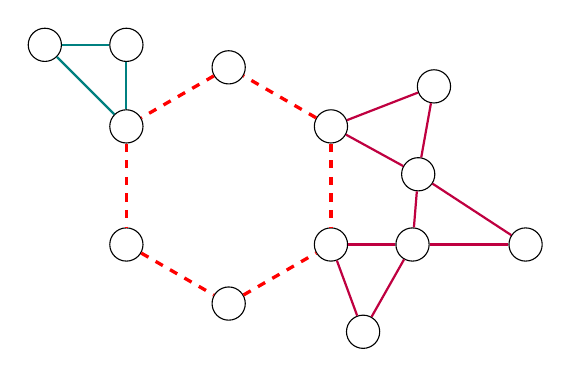
\begin{tikzpicture}[v/.style = {draw, circle, minimum size = 12pt},
    start chain = circle placed {at = (\tikzchaincount*60-30:1.5)},
    every join/.style = {very thick, red, dashed},
    comp/.style = {thick, #1}]
  \foreach \i in {1, ..., 6}
    \node (\i) [v, on chain, join] {};
  \draw [very thick, red, dashed] (1) to (6);

  \node (3a) [v, above = 0.60cm of 3] {};
  \node (3b) [v, left = 0.60cm of 3a] {};
  \path (3) edge[comp = teal] (3a)
	    edge[comp = teal] (3b)
	(3a) edge[comp = teal] (3b);

  \node (1ar) [v, above right = 0.20cm and 1.00cm of 1] {};
  \node (1br) [v, below right = 0.30cm and 0.80cm of 1] {};
  \path (1) edge[comp = purple] (1ar)
  	    edge[comp = purple] (1br)
	(1ar) edge[comp = purple] (1br);

  \node (6r) [v, right = 0.60cm of 6] {};
  \node (6rr) [v, right = 1.00cm of 6r] {};
  \node (6br) [v, below right = 0.80cm and 0.10cm of 6] {};
  \path (6) edge[comp = purple] (6r)
  	    edge[comp = purple] (6br)
	(6r) edge[comp = purple] (6rr)
	     edge[comp = purple] (6br)
	     edge[comp = purple] (1br)
	(1br) edge[comp = purple] (6rr);
\end{tikzpicture}
\end{document}